\chapter{Conclusioni}
\label{chap:conclusioni}
\section{Consuntivo finale}

L'attività di stage ha seguito un piano di lavoro ben definito con obiettivi chiari.
Durante il periodo di stage, ci sono stati momenti di difficoltà che hanno rallentato lo sviluppo.
Le principali problematiche incontrate sono state legate alla gestione della \gls{monorepog}\glox e all'implementazione dell'autenticazione nel \gls{backendg}\glox.
Considero questo periodo molto utile sia per me che per l'azienda, poiché tutto il lavoro svolto ha contribuito a migliorare la gestione di queste problematiche per il futuro.
Ho collaborato attivamente con i membri del team Unox e ogni momento di difficoltà è diventato un'opportunità di discussione costruttiva.
L'obiettivo non era solo risolvere i problemi, ma anche comprenderli e prevenire simili situazioni in futuro.
Lo sviluppo delle pagine richieste è stato valutato positivamente dall'azienda.
Di seguito sono riepilogati gli obiettivi e i requisiti raggiunti:

\subsection{Requisiti raggiunti}


\begin{center}
    \rowcolors{1}{}{tableGray}
    \begin{longtable}{|p{2.25cm}|p{5cm}|}
    \hline
    \multicolumn{1}{|c|}{\textbf{Identificatore}} & \multicolumn{1}{c|}{\textbf{Soddisfatto/non}} \\
    \hline 
    \endfirsthead
    \rowcolor{white}
    \multicolumn{2}{c}{{\bfseries \tablename\ \thetable{} -- Continuazione}}\\
    \hline
    \multicolumn{1}{|c|}{\textbf{Identificatore}} & \multicolumn{1}{c|}{\textbf{Soddisfatto/non}} \\
    \hline 
    \endhead
    \hline
    \rowcolor{white}
    \multicolumn{2}{|r|}{{Continua nella prossima pagina...}}\\
    \hline
    \endfoot
    \endlastfoot
    
    RFN-1 & Soddisfatto  \\
    RFN-2 & Soddisfatto  \\
    RFN-2.1 & Soddisfatto  \\
    RFN-2.2 & Soddisfatto  \\
    RFD-2.2.1 & Soddisfatto  \\
    RFN-3 & Soddisfatto  \\
    RFN-3.1 & Soddisfatto  \\
    RFN-4 & Soddisfatto  \\
    RFN-5 & Soddisfatto  \\
    RFN-5.1 & Soddisfatto  \\
    RFN-5.2 & Soddisfatto  \\
    RFN-5.3 & Soddisfatto  \\
    RFN-6 & Soddisfatto  \\
    RFN-6.1 & Soddisfatto  \\
    RFN-7 & Soddisfatto  \\
    RFN-7.1 & Soddisfatto  \\
    RQN-1 & Soddisfatto  \\
    RQN-2 & Soddisfatto  \\
    RVN-1 & Soddisfatto  \\
    RVN-2 & Soddisfatto  \\
    \hline

    \hiderowcolors
    \caption{Tabella dei requisiti soddisfatti.}
    \label{tab:requisiti_soddisfatti}
    \end{longtable}
\end{center}

\subsection{Raggiungimento degli obiettivi}

\begin{center}
    \rowcolors{1}{}{tableGray}
    \begin{longtable}{|p{5cm}|p{2.75cm}|p{4cm}|}
    \hline
    \multicolumn{1}{|c|}{\textbf{Obiettivo}} & \multicolumn{1}{c|}{\textbf{Tipologia}} & \multicolumn{1}{c|}{\textbf{Raggiunto/non}} \\
    \hline 
    \endfirsthead
    \rowcolor{white}
    \multicolumn{3}{c}{{\bfseries \tablename\ \thetable{} -- Continuazione}}\\
    \hline
    \multicolumn{1}{|c|}{\textbf{Obiettivo}} & \multicolumn{1}{c|}{\textbf{Tipologia}} & \multicolumn{1}{c|}{\textbf{Raggiunto/non}} \\
    \hline 
    \endhead
    \hline
    \rowcolor{white}
    \multicolumn{3}{|r|}{{Continua nella prossima pagina...}}\\
    \hline
    \endfoot
    \endlastfoot
    
    Architettura dell'applicazione & Obbligatorio & Raggiunto  \\
    Autenticazione & Obbligatorio & Raggiunto  \\
    Product Page & Obbligatorio & Raggiunto  \\
    Serviced Oven & Obbligatorio & Raggiunto  \\
    Test piattaforme & Obbligatorio & Raggiunto  \\
    RMA & Desiderabile & Non Raggiunto  \\
    Test E2E & Facoltativo & Non Raggiunto  \\
    \hline

    \hiderowcolors
    \caption{Tabella degli obiettivi raggiunti.}
    \label{tab:obiettivi_raggiunti}
    \end{longtable}
\end{center}

\subsection{Rettrospettiva}

\section{Applicazione consegnata}

\begin{figure}[H]
    \centering
    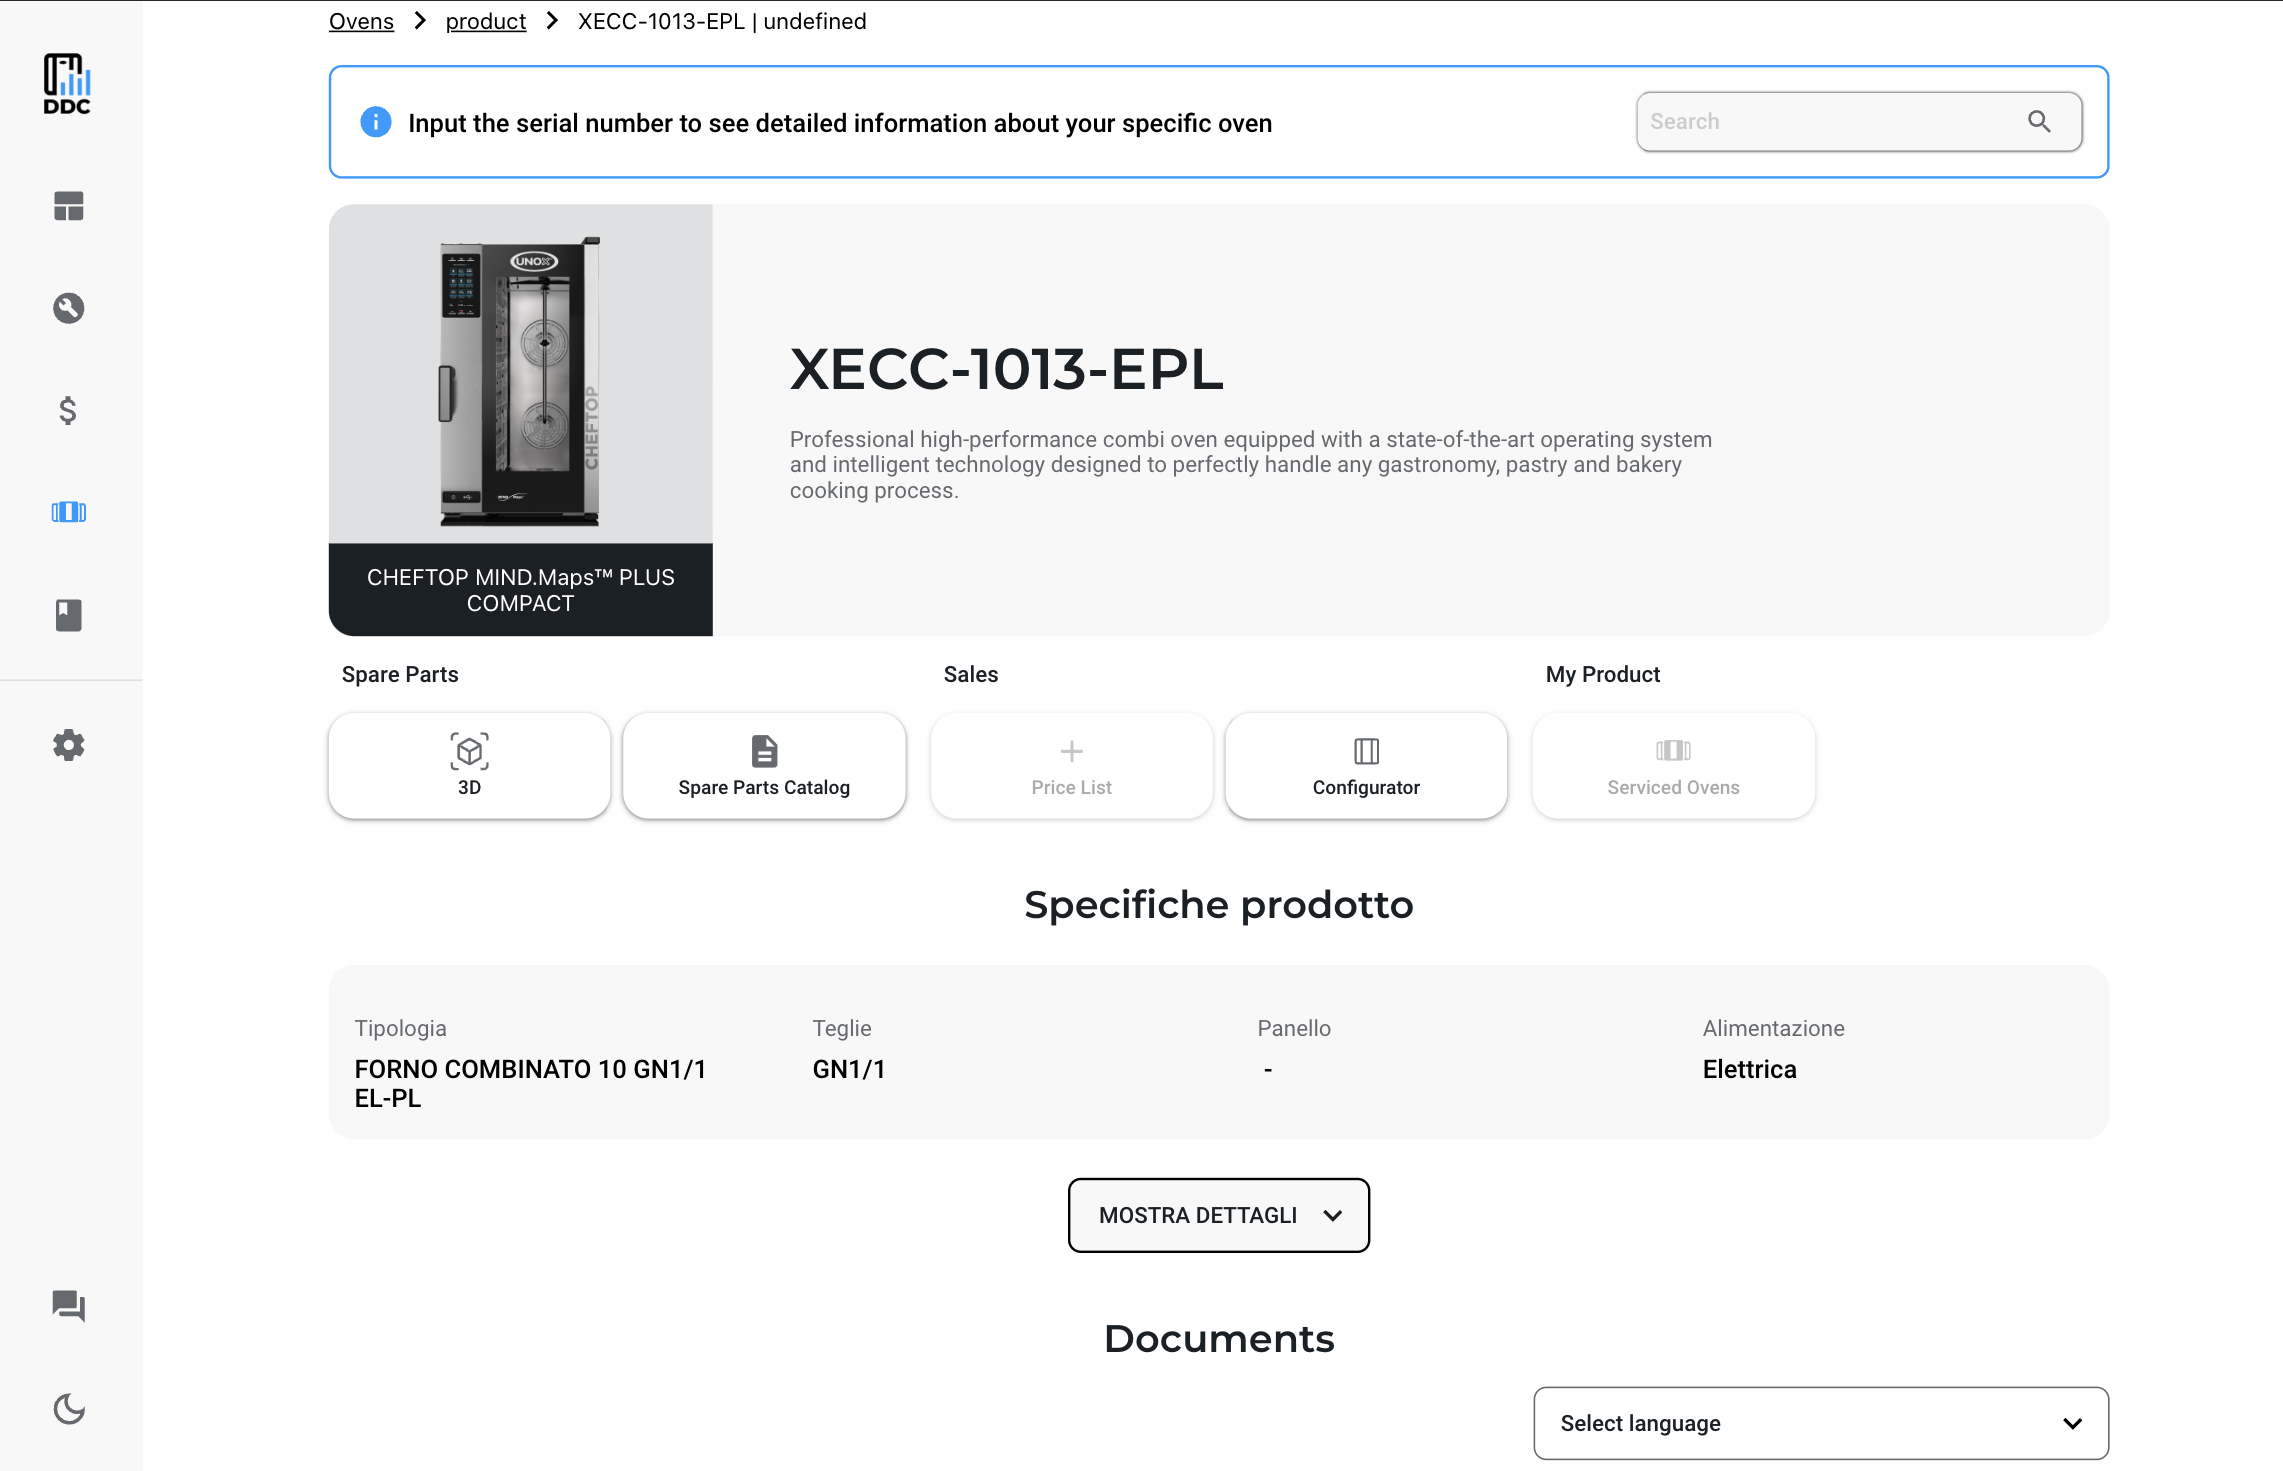
\includegraphics[alt={Screenshot della pagina "Product Page" su piattaforma web}, height=10cm]{img/ProductPageWeb}
    \caption{App \textit{DDC Service} pagina \textit{Product Page} piattaforma \textit{Web}}
    \label{fig:productpageweb}
\end{figure}

\begin{figure}[H]
    \centering
    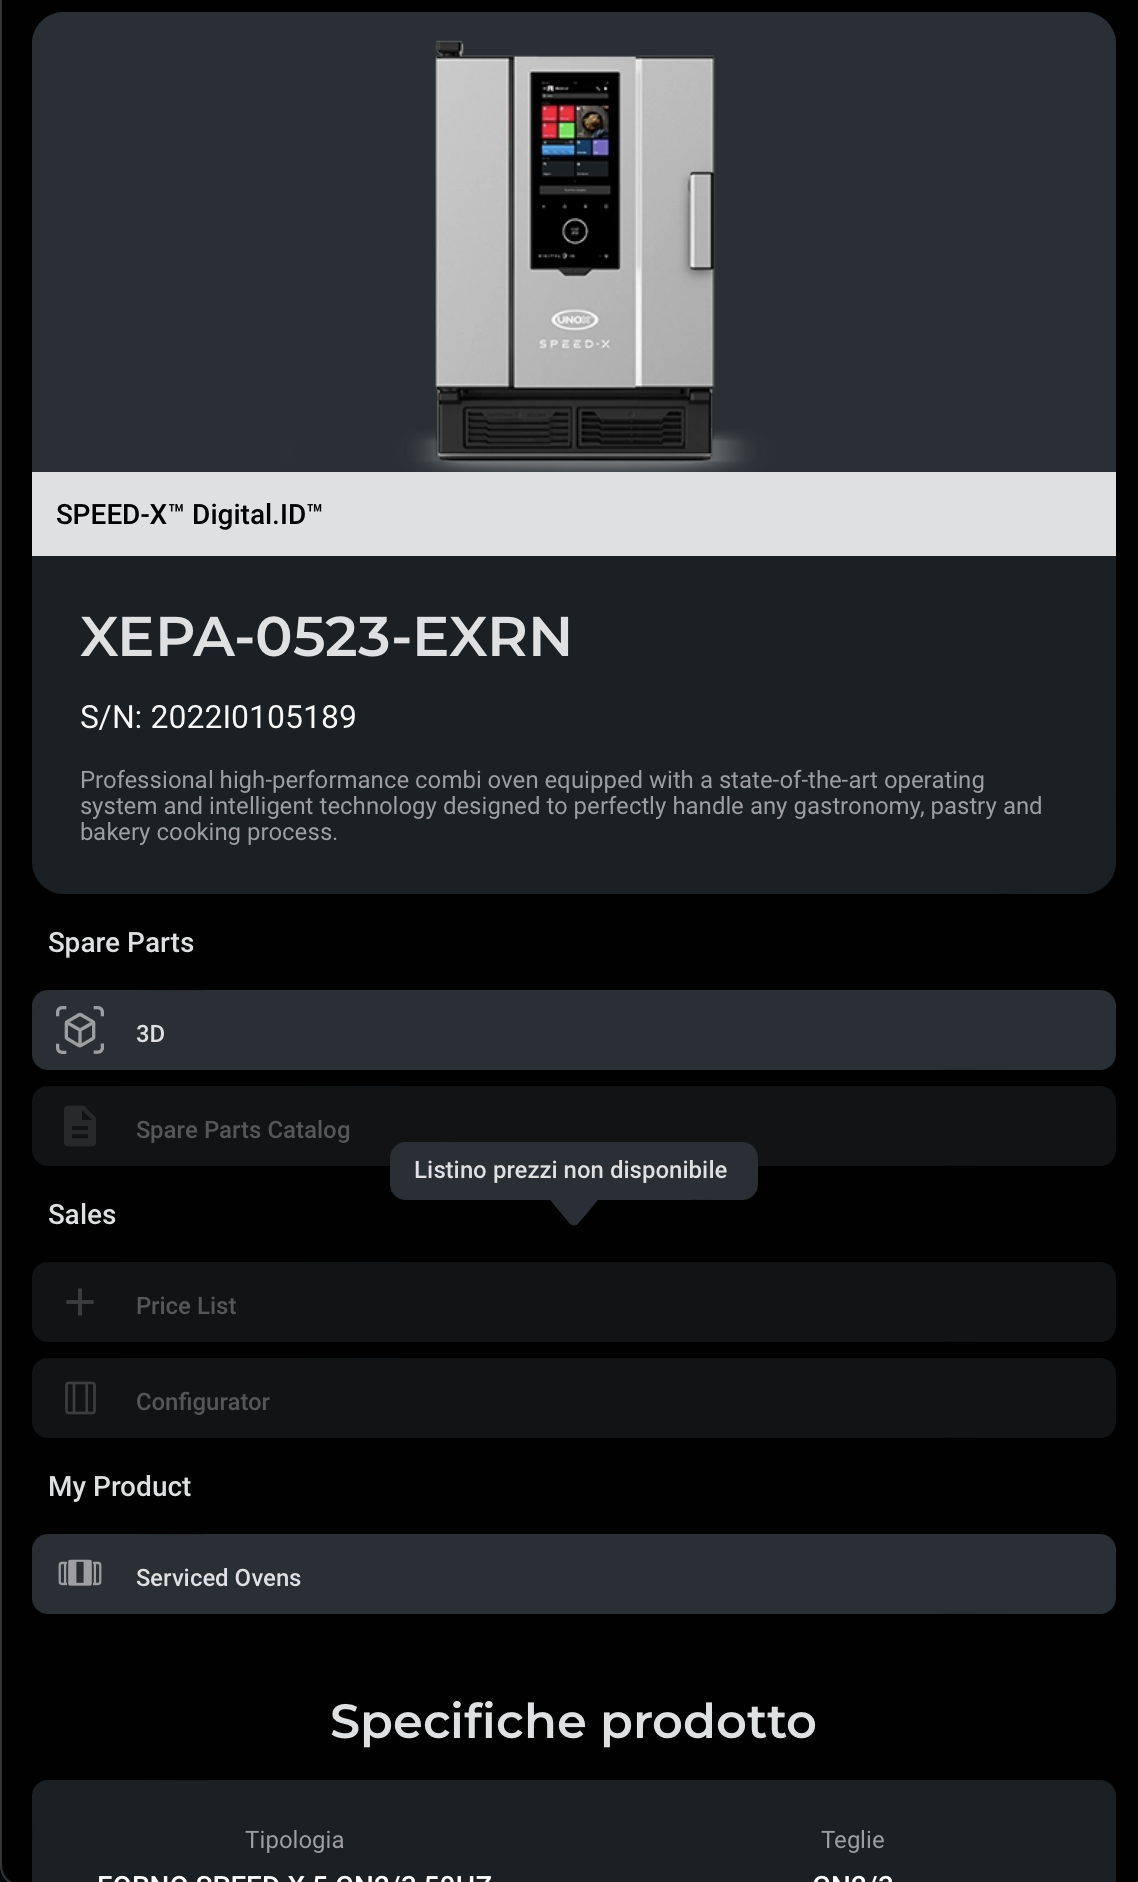
\includegraphics[alt={Screenshot della pagina "Product Page" su piattaforma mobile}, height=15cm]{img/ProductPageMobile}
    \caption{App \textit{DDC Service} pagina \textit{Product Page} piattaforma \textit{Mobile}}
    \label{fig:productpagemobile}
\end{figure}

\begin{figure}[H]
    \centering
    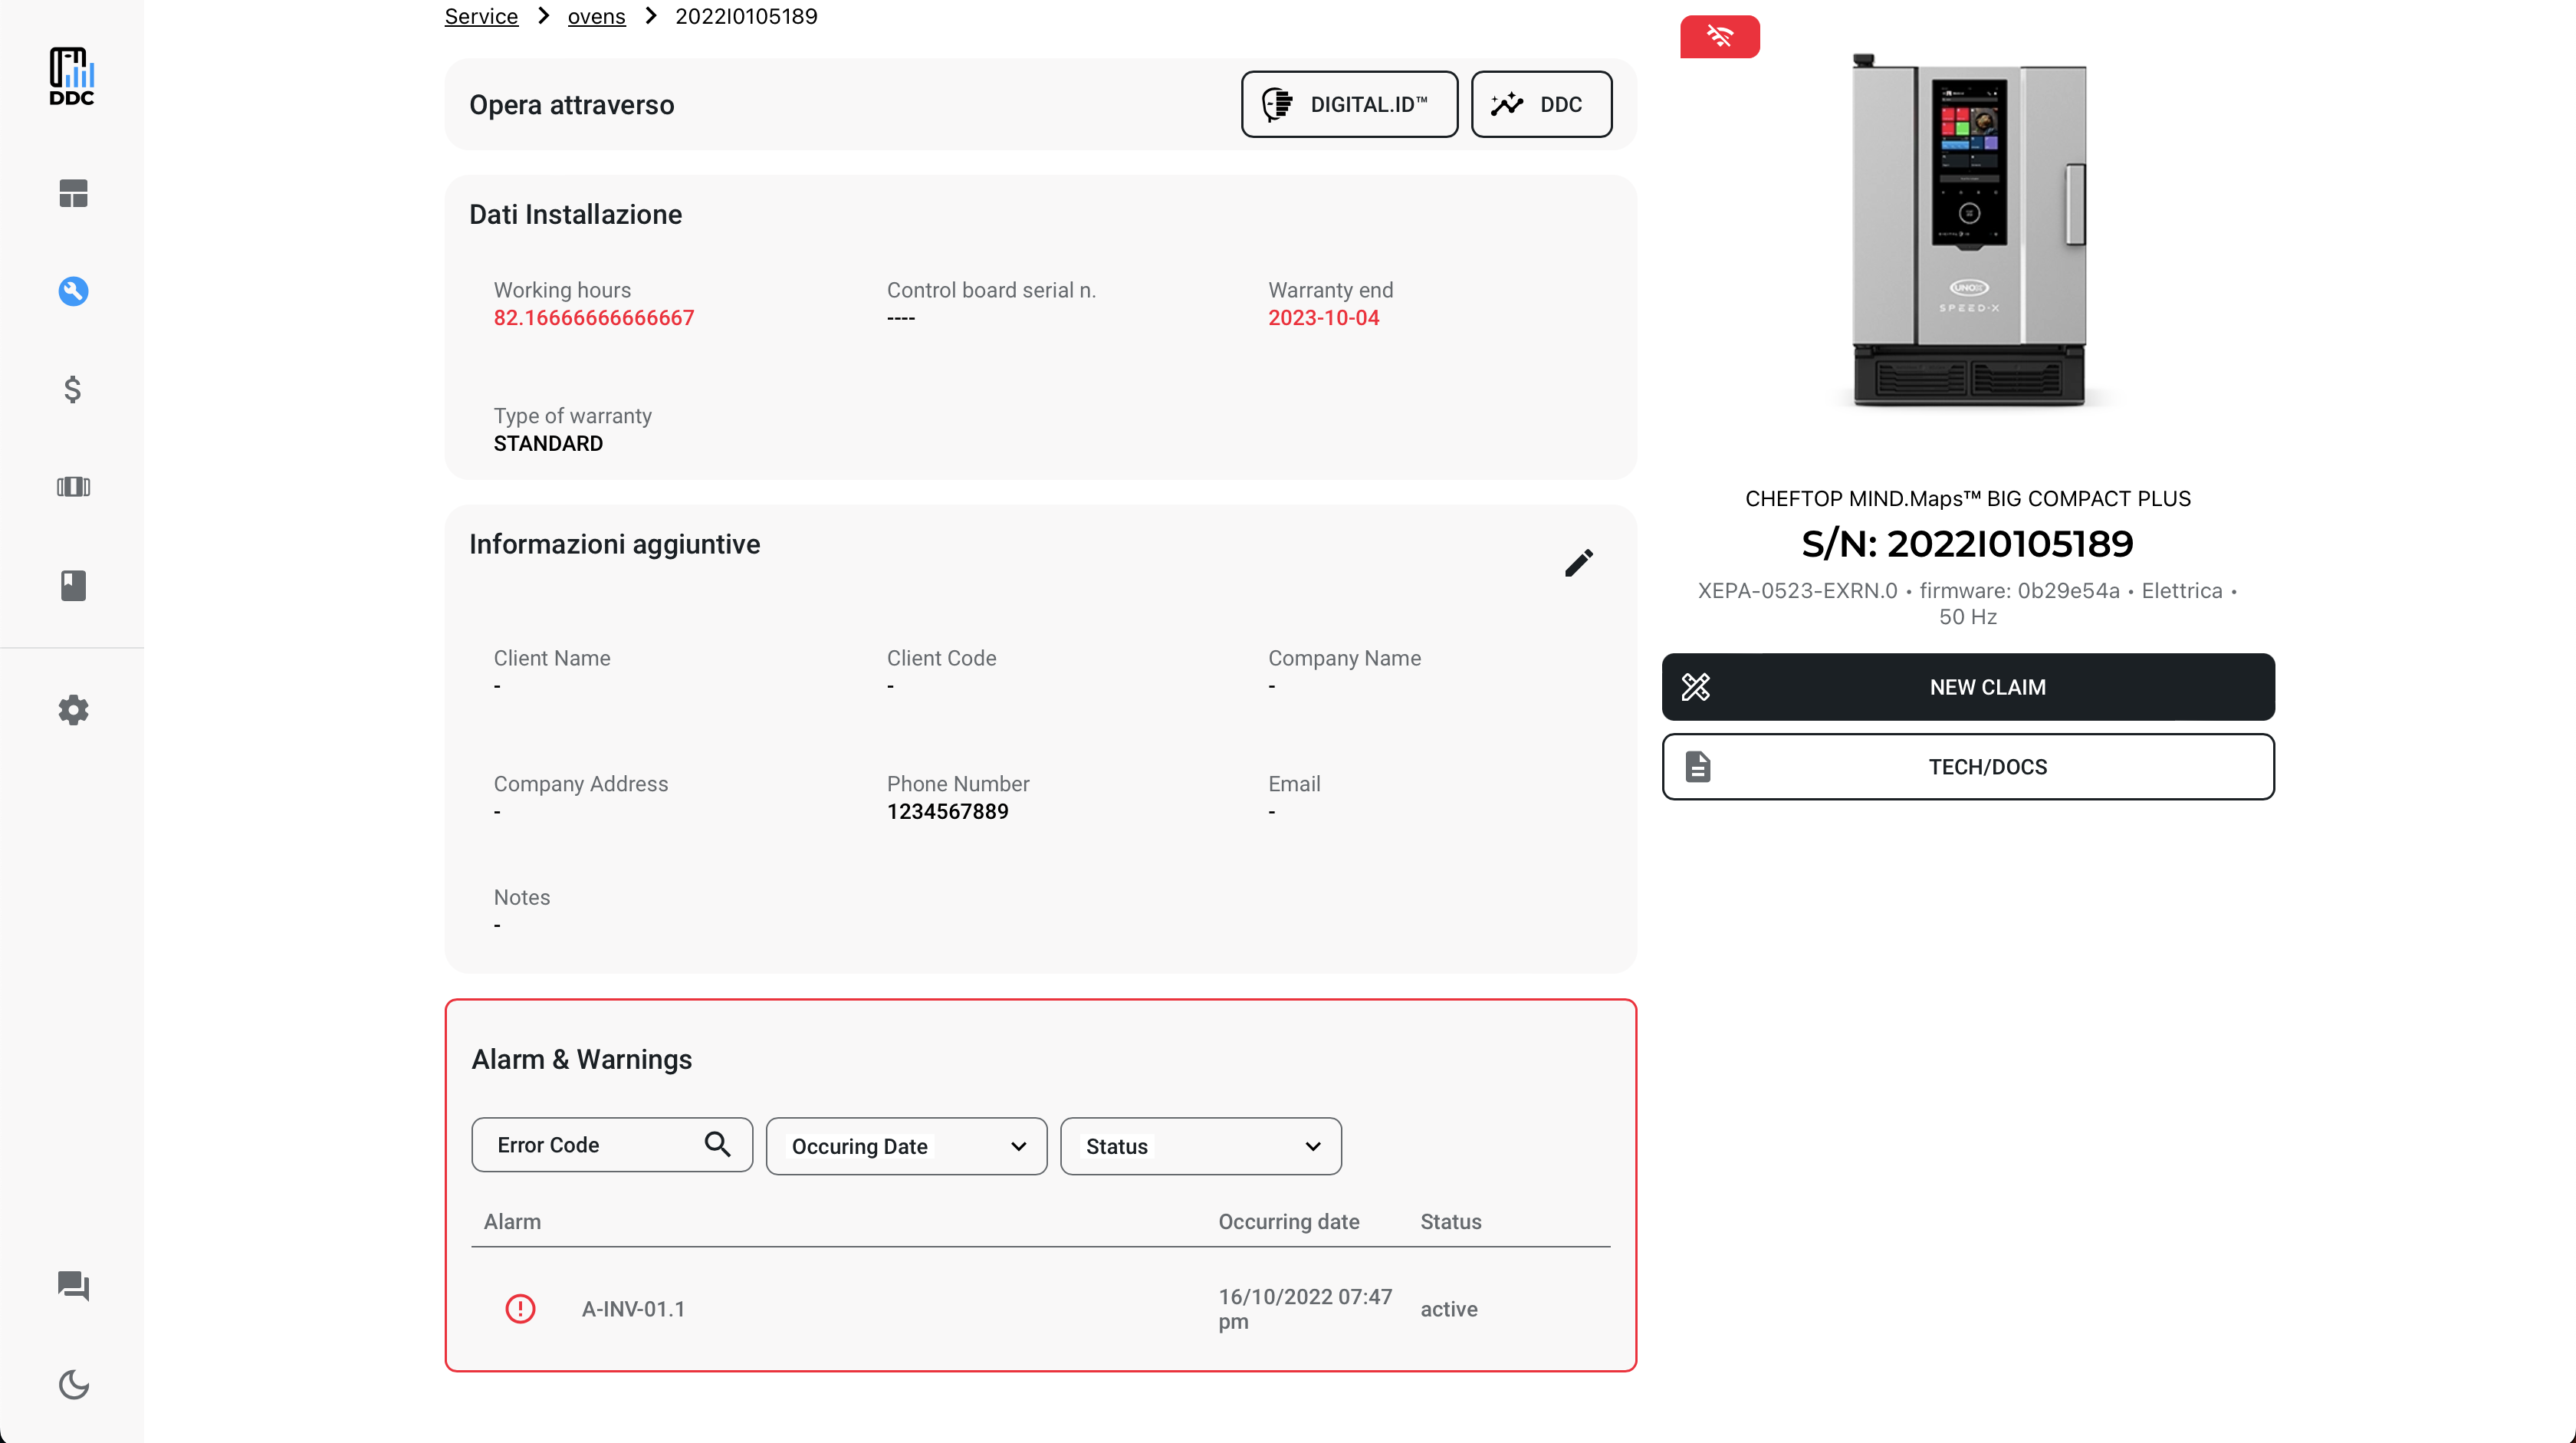
\includegraphics[alt={Screenshot della pagina "Serviced Oven" su piattaforma web}, height=10cm]{img/ServicedOvenWeb}
    \caption{App \textit{DDC Service} pagina \textit{Serviced Oven} piattaforma \textit{Web}}
    \label{fig:servicedovenweb}
\end{figure}



\section{Conoscenze acquisite}

\section{Valutazione personale}

\newpage